\documentclass[11pt,oneside]{book}
\usepackage[T1]{fontenc}
\usepackage[utf8]{inputenc}
\usepackage{lmodern}
\usepackage[margin=1in]{geometry}
\usepackage{amsmath,amssymb,booktabs,longtable,array}
\usepackage{microtype}
\usepackage{xcolor,listings}
\usepackage{graphicx}
\usepackage{pgfplots}
\pgfplotsset{compat=1.18}
\usepackage[hidelinks]{hyperref}
\usepackage{xurl}
\input{version.tex}
\setcounter{tocdepth}{1}
\setlength{\parindent}{0pt}
\setlength{\parskip}{.4em}
\setlength{\emergencystretch}{3em}
\definecolor{VotingGreen}{HTML}{214D35}
\definecolor{ShellOption}{HTML}{7030A0}
\lstdefinestyle{votingbash}{
 language=bash,basicstyle=\ttfamily\footnotesize,
 keywordstyle=\color{VotingGreen}\bfseries,keywordstyle=[2]\color{ShellOption},
 stringstyle=\color{VotingGreen},commentstyle=\color{black!55}\itshape,
 morekeywords={voting,ep,uv,pdflatex},alsoletter={-},
 morekeywords=[2]{--ballot-type,--weight,--type,--seats,--method,--option,
 --choice,--budget,--grade,--approval-limit,--election,--latest,--from,
 --from-results,--register-voters,--abstain,--output-dir,--pdf,--sources-only,
 --allow-expensive,--model,--service,--jobs,--output,--email-trait,--name},
 breaklines=true,breakatwhitespace=true,columns=fullflexible,keepspaces=true,
 frame=single,rulecolor=\color{black!20},backgroundcolor=\color{black!3},
 showstringspaces=false
}
\lstdefinestyle{votingrun}{style=votingbash}
\lstdefinestyle{votingerror}{style=votingbash,rulecolor=\color{orange!70!black}}
\lstset{style=votingbash}
\newcommand{\code}[1]{\texttt{\detokenize{#1}}}
\newcommand{\generated}[1]{\IfFileExists{generated/#1.tex}{\input{generated/#1.tex}}{\begin{quote}\emph{Sources-only edition: execute the example to generate this table or figure.}\end{quote}}}
\newcommand{\ind}{\mathbf{1}}
\title{One Town, Many Ways to Choose\\[.5em]\large A Mathematical and Practical Manual for \texttt{voting}}
\author{The voting project}
\date{First working edition --- September 2026\\Built with voting \VotingVersion}
\begin{document}
\frontmatter
\maketitle
\chapter*{How to use this book}
This book follows one fictional town as it chooses neighborhood projects. The same rankings can favor a library under plurality, shelters under instant runoff, and trees under pairwise comparisons. Rather than declare that one answer is automatically right, we will identify exactly what each rule counts, work through its mathematics, and execute the corresponding commands.

The intended reader is a student, researcher, or practitioner who wants to understand a calculation well enough to challenge it. Familiarity with sums and inequalities is sufficient for most chapters. Graphs appear in the pairwise chapter; a constrained optimization argument appears in the credit chapter. Every symbol is defined before use. Exercises ask readers to calculate, explain, and modify a profile.

\textbf{All preferences in this book are invented teaching data.} The book does not estimate what a real town wants, collect human responses, or execute a language model. Larger weights initially represent groups with identical specified rankings. Later exercises use separate unit-weight panels when the distinction between a weighted agent and repeated people matters.

The manual describes the algorithms implemented by this version of \code{voting}. A method name can cover several variants in the literature. This package makes particular choices about incomplete rankings, lexical ties, weighted quotas, and completion of equal-shares committees. Those choices are stated where they matter. The references provide a route into the wider literature; the executable examples document this implementation.

\section*{Build and inspect}
Install the base package with Python 3.11 or newer and \code{uv}:
\begin{lstlisting}
uv tool install "voting @ git+https://github.com/expectedparrot/voting.git@main"
voting --help
\end{lstlisting}
Then build the book from the installed version:
\begin{lstlisting}
voting docs manual --output-dir town-manual --pdf
voting docs manual --output-dir town-manual-tex
voting docs manual --output-dir town-manual-sources --sources-only
\end{lstlisting}
Choose a new output directory for each build. The first command exports the chapter sources, executes their marked local commands in \code{town-manual/study}, generates numerical tables, and compiles \code{manual.pdf}. The second does everything except PDF compilation. The third exports editable sources without generating numerical results. Source-only PDFs can also be built by adding \code{--pdf}; missing generated material is explicitly labeled.

PDF compilation requires \code{pdflatex}, Latin Modern, PGFPlots, and the standard LaTeX packages in the preamble. It disables shell escape. Local examples require only the base voting package: neither EDSL nor credentials are needed. Instructions for optional human and AI fielding appear in Chapter~\ref{chap:practice}; the build does not execute them.

\code{commands.json} stores exact invocations and JSON envelopes. \code{results.json} contains the saved count results. \code{generated/commands.txt} is the readable transcript, and \code{study/.voting} is an ordinary working project you can inspect. The chapter sources themselves contain the commands the builder executes; there is no hidden ballot generator. Orange command boxes in the validation chapter deliberately produce an error.

Read Chapters 1--4 for single-winner ranked elections, Chapters 5--7 for committees and richer ballots, and Chapter 8 for operating the package. The final chapter and appendices provide a method map, answers to selected exercises, and the command transcript. Generated tables come from actual CLI output; algebraic worked calculations are checked against those results by the manual tests.
\tableofcontents
\mainmatter
\chapter{A town has to choose}
\label{chap:decision}
\section{What is the decision?}
Imagine Alderbrook, a fictional town choosing among four neighborhood proposals: extending Library evening hours, adding bus Shelters, planting street Trees, and improving a Playground. First the town selects one proposal for further development; later it chooses two or three together.

The alternatives are feasible proposals with comparable planning commitments. Selection establishes a priority; it does not authorize construction. A fixed number of winners also differs from a municipal spending limit, especially when project costs vary. Chapter~\ref{chap:credits} returns to that distinction.

A voting rule is a function from recorded messages to an outcome. Before choosing the function, decide who participates, what an option means, what information voters provide, how abstention works, and what a winner authorizes. The most sophisticated aggregation algorithm cannot repair an ambiguous question.

\section{The teaching profile}
We will encode 100 units of voting weight in four groups. Every member of a group has the ranking printed below. The numbers are selected to create an instructive disagreement among methods; they are not observations or estimates.
\begin{center}
\begin{tabular}{lrl}
\toprule Group ID & Weight & Most preferred to least preferred\\\midrule
\code{readers} & 42 & Library $>$ Trees $>$ Shelters $>$ Playground\\
\code{riders} & 26 & Shelters $>$ Playground $>$ Trees $>$ Library\\
\code{canopy} & 17 & Trees $>$ Shelters $>$ Playground $>$ Library\\
\code{families} & 15 & Playground $>$ Shelters $>$ Trees $>$ Library\\
\bottomrule
\end{tabular}
\end{center}
Library has the largest first-choice group. Shelters is a compromise for the two smaller groups. Trees appears above Shelters for the largest group and for its own supporters. These are three different sources of support; the algorithms will give them different roles.

For additive ranked, approval, and score calculations, a row with weight 42 has the same contribution as 42 identical rows of weight one. Grouping saves typing. It does not mean a poll with four actual respondents can be made representative by inventing large weights. When using weights for a real research sample, specify what population or normative role the weights represent.

\section{Notation}
Let $C$ be the set of eligible options, with $m=|C|$. Let $i=1,\ldots,n$ index the latest countable ballot for each participating voter. Ballot $i$ has finite positive weight $w_i$, and total valid weight is
\[
W=\sum_{i=1}^n w_i.
\]
The number of stored rows $n$ and the total weight $W$ are different quantities. Initially $n=4$ and $W=100$. Invalid ballots contribute to neither. An older ballot is superseded when the same voter casts a later ballot in the same election.

For a ranked ballot, $r_i(c)$ is the position of candidate $c$, with position 1 best. Write $a\succ_i b$ when $i$ prefers $a$ to $b$. For approval, $A_i\subseteq C$ is the approved set. For score, $s_i(c)$ is a numeric rating. For grades, $g_i(c)$ is an ordered label. For allocated ballots, $x_i(c)\geq0$ is the number of credits spent on $c$. The symbol $\ind\{P\}$ is 1 if proposition $P$ is true and 0 otherwise.

The number of seats is $k$. It is a count of selected options, not an amount of money. A single-winner rule has $k=1$. Calling an election a budget does not alter the mathematical meaning of seats.

\section{Information comes before aggregation}
A rank says which option is preferred, not how much. Approval records a threshold judgment, not an ordering among approved options. Scores require a common scale. Grades require labels with an agreed ordering. Allocations require a budget and an interpretation of the points.

There is no unique conversion from a ranking into a score vector or an approval set. The same ranking could be produced by almost equal evaluations or by a very intense first preference. Later chapters explicitly supply new invented responses for these instruments. They do not recover those responses from the ranked profile.

The \emph{Handbook of Computational Social Choice} introduces the broader study of preference aggregation.\cite{handbook} Here we develop the rules this package implements.

\section{Exercises}
\begin{enumerate}
\item Without running a command, identify the plurality leader. Why is having the largest group different from having a majority?
\item Count the weight preferring Trees to Shelters. Repeat for Trees against Library. What does this suggest about a rule based on head-to-head contests?
\item Write two score vectors with the Readers ranking but very different gaps between first and second place. Explain why the ranking alone cannot choose between them.
\end{enumerate}

\chapter{Build the election with commands}
\label{chap:project}
\section{Create an ordinary project}
The following listings are executed by the manual build. If working by hand, run the first command from an empty working directory and then enter \code{study}. The builder performs that directory change itself.
\begin{lstlisting}[style=votingrun]
voting init study --description "Alderbrook: fictional teaching elections"
\end{lstlisting}
\begin{lstlisting}
cd study
\end{lstlisting}
Register the four options and four weighted groups. IDs are stable identifiers used in subsequent commands; names are readable labels. A name can contain spaces if quoted.
\begin{lstlisting}[style=votingrun]
voting option add library "Library" --type proposal
voting option add shelters "Shelters" --type proposal
voting option add trees "Trees" --type proposal
voting option add playground "Playground" --type proposal
voting voter add readers "Readers group" --weight 42
voting voter add riders "Bus riders group" --weight 26
voting voter add canopy "Tree supporters" --weight 17
voting voter add families "Playground supporters" --weight 15
\end{lstlisting}
Define an election whose instrument is ranked, attach the eligible choices, and open it. Methods are selected at count time, so there is no \code{--method} on \code{election add}.
\begin{lstlisting}[style=votingrun]
voting election add ranked "One neighborhood priority" --ballot-type ranked
voting election add-option ranked library
voting election add-option ranked shelters
voting election add-option ranked trees
voting election add-option ranked playground
voting election open ranked
\end{lstlisting}

\section{Record preferences}
Arguments after the voter ID are the ranking, best first. The CLI checks that the ballot matches the election's declared type, options exist and are eligible, rankings contain no duplicates, and the voter is eligible.
\begin{lstlisting}[style=votingrun]
voting ballot rank ranked readers library trees shelters playground
voting ballot rank ranked riders shelters playground trees library
voting ballot rank ranked canopy trees shelters playground library
voting ballot rank ranked families playground shelters trees library
voting ballot validate ranked
voting ballot list --election ranked --latest
\end{lstlisting}
Validation should report four valid ballots. It does not report 100 rows: the sum of weights is 100. A weight is captured on the ballot when it is recorded. The current implementation uses that saved ballot weight when counting.

Every command normally emits one JSON envelope with \code{status}, \code{data}, \code{warnings}, \code{errors}, and \code{next_steps}, together with invocation and schema metadata. Most quantities of interest are under \code{data}. Add the top-level flag \code{--human} to display a terminal table:
\begin{lstlisting}
voting --human ballot list --election ranked --latest
\end{lstlisting}
This presentation command is optional; it does not change the stored preferences.

\section{Apply several rules to the same ballots}
\begin{lstlisting}[style=votingrun]
voting count compare ranked
\end{lstlisting}
This prepares one set of valid ballots and runs the compatible methods. Every method's result is saved separately. The comparison gives winner IDs and result IDs, making it possible to inspect a method's full diagnostics with \code{count show}.
\generated{ranked-methods}
The disagreement is the central object of study. Plurality, Borda, elimination, and pairwise comparisons do not use the same summary of the input. The next two chapters derive the summaries and explain the results rather than treating method agreement as a vote among algorithms.

\section{Where the data lives}
\code{study/.voting} contains project metadata, option records, voter records, election definitions, append-only ballot records, and count results. A recast ballot creates a new record. Latest-ballot resolution occurs independently for each election and voter.

Stored counts include the method, seats and settings, winners, ranking, valid and invalid ballot counts, and diagnostics such as rounds or pairwise support. Lightweight provenance includes the used ballot IDs, eligible option IDs, package version, and an input fingerprint. The fingerprint helps detect stale results; it is not a complete frozen copy of all project metadata.

\section{Exercises}
\begin{enumerate}
\item Locate the result ID for IRV in \code{commands.json}, then run \code{voting count show <result_id>} in the study directory. Which fields explain the winner?
\item Why would running an approval counter directly on these ranked ballots be an error? What additional question would you need to ask voters?
\item Interpret a summary with four valid ballots, zero invalid ballots, and total valid weight 100 without describing it as a survey of four representative residents.
\end{enumerate}

\chapter{First choices, positions, and transfers}
\label{chap:ranked}
\section{Plurality and a majority requirement}
Plurality, exposed as \code{fptp}, counts each ballot's first choice:
\[
F(c)=\sum_i w_i\ind\{r_i(c)=1\}.
\]
The option with the greatest $F(c)$ wins. It need not receive more than half the valid weight. In the town profile, Library leads with 42 while the three other first-choice groups sum to 58. That observation alone does not identify which alternative those 58 would choose together.

\code{simple_majority} starts with the same totals but declares a winner only if the highest total is strictly greater than half the total counted first-choice weight. A tie at exactly half is insufficient. When no candidate meets the condition, an empty winner list is an informative outcome, not a software failure.
\begin{lstlisting}[style=votingrun]
voting count run ranked --method fptp
voting count run ranked --method simple_majority
\end{lstlisting}
\begin{center}
\generated{first-choice-plot}
\end{center}
Here and below, L, S, T, and P abbreviate Library, Shelters, Trees, and Playground. The graphic is generated from this build's saved plurality count.

With a single-choice election the input directly supplies the first choice. With a ranked election these two methods extract the first listed option. They do not use lower preferences. This is an intentional compatible reduction of information; a reduction in the opposite direction would be impossible.

\section{Borda: score the position}
With $m$ eligible options, this implementation gives a listed option $m-r_i(c)$ points. For a complete ballot that is $m-1,m-2,\ldots,0$ from best to worst:
\[
B(c)=\sum_{i:\,c\text{ listed}}w_i\bigl(m-r_i(c)\bigr).
\]
For Shelters in the town example,
\[
B(S)=42(1)+26(3)+17(2)+15(2)=184.
\]
For Trees the calculation is $42(2)+26(1)+17(3)+15(1)=176$. Borda rewards positions across all ballots, so the largest first-choice bloc need not control its answer.
\begin{lstlisting}[style=votingrun]
voting count run ranked --method borda
\end{lstlisting}
\generated{ranked-totals}
The columns measure different things. First-choice totals sum to $W=100$. With four completely ranked options, Borda points sum to $W(3+2+1+0)=600$. A Borda total of 184 is not a count of 184 voters or an approval percentage.

For an incomplete ranking, unlisted candidates receive zero in this package while listed candidates keep the points implied by the full eligible option count. Thus listing only a first choice in a four-option election awards it three points, with zero for all others. Other treatments of truncated ballots exist. Record this convention when comparing implementations.

\section{Instant runoff voting}
IRV maintains an active set $C_t$, initially $C$. Let $h_i(C_t)$ be the first listed candidate on ballot $i$ who remains active. If none remains, the ballot is exhausted in that round. Define
\[
F_t(c)=\sum_i w_i\ind\{h_i(C_t)=c\},\qquad
W_t=\sum_{c\in C_t}F_t(c).
\]
The algorithm is:
\begin{enumerate}
\item Count first active choices and record exhausted weight.
\item If a candidate has $F_t(c)>W_t/2$, elect it and stop. If only one candidate remains, elect that candidate.
\item Otherwise eliminate a candidate with the lowest $F_t(c)$, remove it from $C_t$, and repeat.
\end{enumerate}
When the lowest totals tie, the package eliminates the lexicographically smallest tied ID. The same rule favoring a smaller ID for a winning tie therefore removes a smaller ID in an elimination tie. Determinism is useful for replication, but the direction of the tie operation matters.
\begin{lstlisting}[style=votingrun]
voting count run ranked --method irv
\end{lstlisting}
\generated{irv-rounds}
Playground is eliminated first. Its 15 units transfer to Shelters, taking Shelters to 41. Trees is then the lowest active candidate with 17; that group's next surviving option is Shelters. Shelters reaches 58 and wins against Library's 42.

Notice the difference between a transfer and a new vote. The Families ballot is counted for exactly one active candidate at a time. It does not continue contributing to Playground after transferring. IRV reallocates the original weight; it does not add weight each round.

Incomplete rankings can exhaust. If a voter lists only Playground, its elimination removes that ballot's weight from $W_t$. A majority of continuing weight can therefore be smaller than a majority of the original electorate. Inspect \code{exhausted_weight} and round totals when interpreting such an outcome.

IRV stops when a winner is found. Its remaining non-winner order is a presentation convention: active candidates follow in their final tally order, then eliminated candidates in reverse elimination order. Do not interpret that displayed order as the result of conducting a fresh runoff for every lower position.

\section{Bucklin: widen the accepted depth}
Bucklin also uses rankings, but it accumulates support at increasing depths instead of eliminating candidates:
\[
D_\ell(c)=\sum_i w_i\ind\{c\text{ appears among the first }\ell\text{ positions of }i\}.
\]
Start at $\ell=1$ and increase it until some $D_\ell(c)>W/2$. Among candidates meeting that condition at the first successful depth, the package selects the largest $D_\ell(c)$, then the larger previous-depth total, then the smaller ID.

At depth two in Alderbrook, Trees receives the Readers' 42 and its own 17, for 59. Shelters receives 26 from Riders, 17 from Canopy, and 15 from Families, for 58. Both cross 50 at that depth, and Trees wins by one unit of accumulated support.
\begin{lstlisting}[style=votingrun]
voting count run ranked --method bucklin
\end{lstlisting}
Depth-two totals can sum to $2W$ on complete ballots. Unlike IRV, the same ballot contributes to two candidates at this depth. This is not double-counting within Bucklin; it is the defined statistic.

On truncated ballots a majority might never emerge. The implementation then uses the largest accumulated support at the final depth, breaking ties by ID. If a research design requires no winner in that situation, that is a different fallback rule.

\section{A simulated two-round runoff}
The \code{runoff} method selects the two largest first-choice totals, then counts each ranked ballot for whichever finalist it ranks first. In our profile the finalists are Library and Shelters, and the final comparison is 42 to 58.
\begin{lstlisting}[style=votingrun]
voting count run ranked --method runoff
\end{lstlisting}
This package always constructs the two stages, even if the first-stage leader already has a majority. With complete rankings such a leader necessarily also beats the other finalist. With single-choice ballots, a voter whose chosen option misses the final has no recorded fallback and contributes to \code{no_preference}. The simulated runoff then cannot measure how those voters would behave in a second election.

Even ranked ballots do not observe an actual second campaign. Turnout, information, and preferences may change between real rounds. Describe this computation as a runoff simulated from the recorded preference profile.

\section{Exercises}
\begin{enumerate}
\item Verify that the four Borda totals sum to 600. Explain why the analogous sum changes with truncated ballots.
\item If all Families ballots list only Playground, compute the continuing weight after its elimination. Follow the remaining rounds and report both the winner and exhausted weight.
\item Explain why a Bucklin depth-two total of 59 and an IRV final total of 58 refer to different coalitions and cannot be compared as measurements of the same quantity.
\end{enumerate}

\chapter{Compare every pair}
\label{chap:pairwise}
\section{The pairwise matrix}
Define the directed support matrix
\[
P(a,b)=\sum_iw_i\ind\{a\succ_i b\},\qquad a\ne b.
\]
For complete strict rankings, $P(a,b)+P(b,a)=W$. A candidate $a$ beats $b$ when $P(a,b)>P(b,a)$. A \emph{Condorcet winner} beats every other candidate in these head-to-head comparisons.

The package treats a listed option as preferred to an unlisted one. If both are unlisted, that ballot contributes to neither direction for that pair. Consequently, incomplete ballots can give $P(a,b)+P(b,a)<W$. There is no ranked-ballot syntax for explicit tied positions among listed options.
\generated{pairwise}
Each entry counts the weight preferring the row to the column. Trees beats Library 58 to 42, Shelters 59 to 41, and Playground 59 to 41. It is therefore the Condorcet winner, even though IRV eliminated it. The disagreement is not a numerical mistake: elimination and pairwise dominance are different rules.

A pairwise margin is $M(a,b)=P(a,b)-P(b,a)$. Do not confuse a support of 59 with a margin of 18. Different Condorcet extensions rank or compare these quantities differently.

\section{Copeland and minimax}
\code{copeland} assigns one point for a pairwise win, half a point for a tie, and zero for a loss:
\[
K(a)=\sum_{b\ne a}\left(\ind\{P(a,b)>P(b,a)\}
             +\tfrac12\ind\{P(a,b)=P(b,a)\}\right).
\]
It orders candidates by decreasing $K(a)$, then ID. These are points for contests, not total voter support. A narrow win and a large win each contribute one point.

\code{minimax} instead measures the worst positive defeat margin:
\[
D(a)=\max\left(0,\max_{b\ne a}\{P(b,a)-P(a,b)\}\right).
\]
It favors the smallest $D(a)$; saved scores are $-D(a)$ so that higher remains better. An undefeated candidate has zero worst defeat. This is the margins variant, not a variant based on the opponent's raw winning votes.
\begin{lstlisting}[style=votingrun]
voting count run ranked --method copeland
voting count run ranked --method minimax
\end{lstlisting}
Trees wins both. To learn how these rules differ, one needs a profile without a Condorcet winner, rather than repeatedly recounting a profile on which that criterion resolves the choice.

\section{Ranked pairs: lock strong victories}
Construct one directed edge $a\to b$ for every strict pairwise victory. Sort these victories by decreasing margin, then decreasing winning support, then the winner and loser IDs. Start with an empty directed graph.
\begin{enumerate}
\item Consider each victory in the sorted order.
\item Before adding $a\to b$, check whether a directed path already runs from $b$ to $a$.
\item If it does, skip this edge: adding it would create a cycle. Otherwise lock the edge.
\item After all victories have been considered, take a topological ordering of the locked graph. Choose the first candidate.
\end{enumerate}
A topological order places the winner of every locked edge before its loser. In this implementation, when several candidates have no remaining incoming edge, the smallest ID is selected next. Merely counting outgoing minus incoming edges does \emph{not} preserve the constraints of the locked graph.

The source-node characterization of ranked-pairs winners is also used in research on its computational properties.\cite{rankedpairs} Here \code{locked} records accepted edges, and \code{skipped} records those rejected to avoid a cycle.
\begin{lstlisting}[style=votingrun]
voting count run ranked --method ranked_pairs
\end{lstlisting}

\section{Schulze: compare strongest paths}
Schulze uses a different graph calculation. Initialize the strength of a direct path as
\[
p(a,b)=
\begin{cases}
P(a,b),&P(a,b)>P(b,a),\\
0,&\text{otherwise}.
\end{cases}
\]
The strength of a multi-edge path is the minimum edge strength along it. The strongest path between two candidates maximizes that bottleneck over possible paths. For every intermediate candidate $h$, update distinct $a,b,h$ by
\[
p(a,b)\leftarrow
\max\left(p(a,b),\min\{p(a,h),p(h,b)\}\right).
\]
This is a max--min analogue of the Floyd--Warshall dynamic program. It needs $O(m^3)$ updates after the pairwise matrix has been built; it does not enumerate every path separately.

The implementation orders candidates by the number of opponents for which $p(a,b)>p(b,a)$, then lexicographically. It returns the strongest-path matrix as \code{path_strengths}. The name \code{beatpath} is an alias. Schulze's own exposition gives the broader definition, examples, and variants.\cite{schulze}
\begin{lstlisting}[style=votingrun]
voting count run ranked --method schulze
\end{lstlisting}
An indirect path does not imply that the same voters support every edge. The method aggregates pairwise information; it does not discover a single transitive coalition that submitted the full path.

\section{Kemeny--Young: optimize a complete order}
For a proposed complete ordering $\pi=(\pi_1,\ldots,\pi_m)$, define
\[
J(\pi)=\sum_{1\leq j<\ell\leq m}P(\pi_j,\pi_\ell).
\]
Each term rewards agreement between the proposed social order and the recorded pairwise preferences. Kemeny--Young chooses an order maximizing $J$ and elects its first candidate. This implementation breaks an exact optimum tie by choosing the lexicographically smallest order.
\begin{lstlisting}[style=votingrun]
voting count run ranked --method kemeny_young
\end{lstlisting}
The implementation enumerates all $m!$ orders and scores each in $O(m^2)$ work. Four options require only 24 orders. Nine require 362,880, while twelve require 479,001,600. Default comparisons skip this method above nine eligible options, and explicit runs above that limit require \code{--allow-expensive}. The flag changes a resource guard, not the mathematical rule or computational complexity.

\section{A cycle laboratory}
Consider three additional, unit-weight teaching voters. Their preferences form a symmetric cycle. These ballots live in a separate election so the main profile remains available for comparison.
\begin{lstlisting}[style=votingrun]
voting voter add cycle_1 "Cycle voter 1"
voting voter add cycle_2 "Cycle voter 2"
voting voter add cycle_3 "Cycle voter 3"
voting election add cycle "Three-way cycle" --ballot-type ranked
voting election add-option cycle library
voting election add-option cycle shelters
voting election add-option cycle trees
voting election open cycle
voting ballot rank cycle cycle_1 library shelters trees
voting ballot rank cycle cycle_2 shelters trees library
voting ballot rank cycle cycle_3 trees library shelters
voting count compare cycle
\end{lstlisting}
Library beats Shelters, Shelters beats Trees, and Trees beats Library, each by 2 to 1. Individual rankings are transitive, yet majority comparisons are cyclic. No Condorcet winner exists.
\generated{cycle-methods}
Here some outputs depend on tie conventions because the construction is deliberately symmetric. A winning ID in such a profile is not evidence of stronger underlying support. Rename the options in a fresh copy and preserve the same preference relationships to investigate that dependence.

\section{Exercises}
\begin{enumerate}
\item Compute Trees' Copeland score and minimax score in the town profile.
\item In the three-way cycle, write the ranked-pairs edges in the order considered by the package. Which edge is skipped?
\item What is the strongest path from Library to Trees in the cycle? Compare its strength with the reverse strongest path.
\item Explain why a graph's topological ordering is not obtained by sorting each node's number of wins minus losses.
\end{enumerate}

\chapter{Choose a committee}
\label{chap:committees}
\section{Several seats change the objective}
Selecting $k$ projects is not simply selecting a single winner $k$ times. A top-$k$ score rule rewards the largest totals; a transfer or budget-sharing rule can reduce the influence already used to elect one candidate. Neither approach is universally appropriate. A shortlist of the strongest standalone proposals and a committee intended to represent different constituencies answer different questions.

The CLI checks the seat capabilities of a method. Running Borda with two seats is rejected; its implementation is single-winner. STV, approval, block voting, limited voting, SNTV, cumulative, quadratic, and equal shares support multiple seats. A default comparison skips methods that cannot honor the requested settings and reports the reason.

\section{STV: retain a quota, transfer the surplus}
For $k>1$, this package's STV implementation uses a Droop quota
\[
Q=\left\lfloor\frac{W}{k+1}\right\rfloor+1.
\]
Initially each ballot carries its original weight. Each round assigns its current weight to its first active ranked candidate. If candidate $c$ has total $T(c)\geq Q$, elect it. Its surplus is $T(c)-Q$; each ballot assigned to it is scaled by
\[
f(c)=\frac{T(c)-Q}{T(c)}.
\]
Removing $c$ from the active set lets that residual weight move to the next surviving preference in the next round. Exactly $Q$ of the assigned weight is retained when $T(c)>0$. If $T(c)=Q$, those ballots have no residual transferable weight.

If several candidates meet quota in a round, the package processes them by descending tally and then ID, using that round's assignments. If none meets quota, it eliminates the lowest tally. When the remaining active candidates exactly fill the unfilled seats, it elects them without requiring quota. This is a fractional-surplus STV variant; it is not a claim to reproduce every jurisdiction's transfer procedure.
\begin{lstlisting}[style=votingrun]
voting count run ranked --method stv --seats 2
\end{lstlisting}
For the main profile, $Q=\lfloor100/3\rfloor+1=34$. Library begins with 42 and transfers a surplus of 8 to Trees. Its multiplier is $8/42$. Trees then has 25, Shelters 26, and Playground 15. Eliminating Playground transfers 15 to Shelters, which reaches 41 and takes the second seat.
\generated{stv-rounds}
The displayed totals in successive rounds need not sum to the original $W$: weight has been retained by already elected candidates. Exhausted residual weight is a different reason for a reduced continuing total.

For one seat, \code{stv} dispatches to IRV. The floor in the multi-seat quota makes arbitrary rescaling of fractional weights consequential: multiplying all weights by a constant is not generally equivalent to changing the unit of measurement. Use integer multiplicities when intending weighted rows to represent repeated people in a quota calculation, and state the chosen units.

\section{SNTV: one mark, several winners}
Single non-transferable vote selects the $k$ largest single-choice totals. Votes for a winning candidate are not transferred, and votes for a losing candidate receive no fallback. To illustrate it honestly, create a separate single-choice instrument, using the original profile's first choices as an explicitly disclosed reduction.
\begin{lstlisting}[style=votingrun]
voting election add first_choices "Two projects from first choices" --ballot-type single_choice --seats 2
voting election add-option first_choices library
voting election add-option first_choices shelters
voting election add-option first_choices trees
voting election add-option first_choices playground
voting election open first_choices
voting ballot cast first_choices readers --choice library
voting ballot cast first_choices riders --choice shelters
voting ballot cast first_choices canopy --choice trees
voting ballot cast first_choices families --choice playground
voting count run first_choices --method sntv
\end{lstlisting}
Library and Shelters take the two seats, as they did under STV here. Agreement on one profile does not imply equivalence. Change how many supporters concentrate on one candidate and STV's surplus transfer may matter.

\section{Approval and block voting}
An approval tally is
\[
A(c)=\sum_i w_i\ind\{c\in A_i\}.
\]
With $k$ seats, this implementation elects the $k$ largest totals. Each ballot may contribute to several candidates, but never more than once to the same candidate. A valid empty approved set contributes zero everywhere and remains a recorded abstention.

The following approval sets are new teaching assumptions. In particular, which options cross an approval threshold cannot be read uniquely from the rankings.
\begin{lstlisting}[style=votingrun]
voting election add approvals "Which projects are acceptable?" --ballot-type approval
voting election add-option approvals library
voting election add-option approvals shelters
voting election add-option approvals trees
voting election add-option approvals playground
voting election open approvals
voting ballot approve approvals readers --option library --option trees
voting ballot approve approvals riders --option shelters --option playground --option trees
voting ballot approve approvals canopy --option trees --option shelters
voting ballot approve approvals families --option playground --option shelters
voting count compare approvals
\end{lstlisting}
\generated{approval-methods}
Trees is approved by 85 units of weight, Shelters by 58, Playground by 41, and Library by 42. These approval percentages have a different denominator interpretation from Borda points. The sum of approvals can exceed $W$ because people may approve several options.

\code{block_voting} uses the same totals but permits at most $k$ approvals per ballot, or a stricter election-level limit. It is therefore a constrained ballot format followed by a top-$k$ count. The current three-option Riders ballot is compatible with a three-seat block election:
\begin{lstlisting}[style=votingrun]
voting count run approvals --method block_voting --seats 3
\end{lstlisting}
It is not compatible with a one-seat block election. That is why the earlier default one-seat comparison skips block voting rather than silently discarding approved options.

\section{Limited voting}
Limited voting gives a voter at most $\ell$ approvals, where $1\leq\ell<k$. It again selects the $k$ largest approval totals. The smaller per-voter limit changes what coalitions can support simultaneously; it does not itself guarantee a particular representative composition.
\begin{lstlisting}[style=votingrun]
voting election add limited "Three places, two approvals each" --ballot-type approval --seats 3 --approval-limit 2
voting election add-option limited library
voting election add-option limited shelters
voting election add-option limited trees
voting election add-option limited playground
voting election open limited
voting ballot approve limited readers --option library --option trees
voting ballot approve limited riders --option shelters --option playground
voting ballot approve limited canopy --option trees --option shelters
voting ballot approve limited families --option playground --option shelters
voting count compare limited
\end{lstlisting}
\generated{limited-methods}
Here approval, block, and limited counts use the same legal ballots, so their selected sets coincide. This is useful: it reveals that their distinction lies in permitted messages, not three different formulas applied to these messages. The Riders response differs from the earlier unconstrained approval response; it is an explicit new answer to a stricter question.

Without a configured limit, the limited-voting counter uses $k-1$ and requires at least two seats. Setting \code{--approval-limit} before collection also enforces that constraint on direct entry and hosted approval questions.

\section{Exercises}
\begin{enumerate}
\item Verify that Library retains exactly 34 units when its STV surplus transfers.
\item Why should the second elected member of a three-seat committee not be called the runner-up? The comparison output uses the first unelected candidate instead.
\item Construct a profile where SNTV gives two seats to a large bloc's candidates. Redistribute that bloc's single-choice votes without changing its size. Does the result change?
\end{enumerate}

\chapter{Scores, runoffs, and grades}
\label{chap:cardinal}
\section{What a score means}
A score ballot records numeric evaluations. Summing them requires treating the stated units as comparable across voters. Choosing 0--10 rather than 0--5 is not the main issue: uniformly rescaling everyone preserves a sum ordering, while changing one person's use of the scale changes their relative influence.

The CLI requires finite numeric scores but imposes no default minimum or maximum. Hosted score surveys currently ask for integers from 0 to 10. Our example follows that scale deliberately; it is not a promise that arbitrary imported scores will be range-checked.

\section{Score voting}
The score counter chooses the largest weighted total,
\[
S(c)=\sum_{i:\,c\text{ scored}}w_i s_i(c).
\]
Missing scores contribute zero to this total. The displayed average is
\[
\bar s(c)=\frac{S(c)}{\sum_{i:\,c\text{ scored}}w_i},
\]
when that denominator is positive. This average is descriptive: it is not the selection criterion. With different patterns of missing scores, the average ordering can differ from the total ordering.
\begin{lstlisting}[style=votingrun]
voting election add scores "Support on a zero-to-ten scale" --ballot-type score
voting election add-option scores library
voting election add-option scores shelters
voting election add-option scores trees
voting election add-option scores playground
voting election open scores
voting ballot score scores readers library=10 shelters=2 trees=7 playground=0
voting ballot score scores riders library=0 shelters=10 trees=5 playground=6
voting ballot score scores canopy library=0 shelters=8 trees=10 playground=3
voting ballot score scores families library=0 shelters=7 trees=5 playground=10
voting count compare scores
\end{lstlisting}
\generated{score-totals}
These evaluations happen to preserve each group's original strict ranking. Their distances are additional assumptions. Trees' high score total reflects the Readers' substantial second-choice support as well as its own group's enthusiasm.

Before studying strategic score submission, distinguish a behavioral question from an arithmetic fact. Maximizing one's influence under a sum can favor extreme reports in some settings. A table of sincere-looking fictional scores is not evidence that people will submit them under strategic incentives.

\section{STAR: score, then automatic runoff}
STAR first chooses the two candidates with the largest score totals. For finalists $a,b$, define
\[
R(a,b)=\sum_i w_i\ind\{s_i(a)>s_i(b)\}.
\]
Each voter contributes its full weight to whichever finalist it scores higher. Equal scores contribute to neither direction and are recorded as no preference. Missing finalist scores are treated as zero by this implementation.

The greater runoff total determines the winner. Thus one point of score difference and ten points both express one directional preference in the second stage. The score gap matters for reaching the final, but not for the weight of the final preference.
\generated{star-runoff}
The package implements the two-stage idea with lexicographic tie handling and unrestricted direct-entry scores. Published STAR specifications use a prescribed scale and richer tie procedures; do not claim exact conformance to those specifications from the shared method name alone.\cite{star}

\section{A score winner can lose the runoff}
To see the distinction, use a separate five-person panel considering Library, Shelters, and Trees. Unit weights make every arithmetic step visible. These people and scores are additional invented examples, not a disaggregation of the original four groups.
\begin{lstlisting}[style=votingrun]
voting voter add star_1 "STAR voter 1"
voting voter add star_2 "STAR voter 2"
voting voter add star_3 "STAR voter 3"
voting voter add star_4 "STAR voter 4"
voting voter add star_5 "STAR voter 5"
voting election add star_demo "Score versus final preference" --ballot-type score
voting election add-option star_demo library
voting election add-option star_demo shelters
voting election add-option star_demo trees
voting election open star_demo
voting ballot score star_demo star_1 library=5 shelters=4 trees=0
voting ballot score star_demo star_2 library=5 shelters=3 trees=0
voting ballot score star_demo star_3 library=0 shelters=5 trees=4
voting ballot score star_demo star_4 library=0 shelters=5 trees=3
voting ballot score star_demo star_5 library=3 shelters=2 trees=5
voting count compare star_demo
\end{lstlisting}
\generated{star-reversal}
Shelters has score total 19, Library 13, and Trees 12. Library reaches the final and is preferred to Shelters by voters 1, 2, and 5, so it wins 3 to 2. A correct result must show Library as elected in both its winner field and final ranking, while preserving the score totals as a separate diagnostic.

\section{Majority judgment}
Grades are ordered categories rather than numeric distances. Let the scale be $G_0<G_1<\cdots<G_q$. The package defaults to reject, poor, fair, good, excellent. A monotone relabeling preserves the ordering; there is no assumption that the distance from fair to good equals that from good to excellent.

For candidate $c$, let $H_c(j)$ be the total weight assigning grade $G_j$, and let $W_c=\sum_jH_c(j)$ include only voters who graded $c$. The lower weighted median is the smallest grade index satisfying
\[
2\sum_{j=0}^{h}H_c(j)\ \geq\ W_c.
\]
For two equally weighted grades reject and excellent, this convention returns reject. It does not average them into fair. A candidate with no grades has no median and sorts below graded candidates.

Candidates are compared first by median grade. If tied, remove one median unit from each tied distribution and compare the medians again, repeating as necessary. Decimal weights are represented internally by exact integer units on a common denominator, so fractional weights are not rounded down to zero and large weights do not require repeated ballot objects. Identical remaining distributions are finally ordered by ID. See Balinski and Laraki for the median-removal approach.\cite{majorityjudgment}
\begin{lstlisting}[style=votingrun]
voting election add grades "Project grades" --ballot-type grade
voting election add-option grades library
voting election add-option grades shelters
voting election add-option grades trees
voting election add-option grades playground
voting election open grades
voting ballot grade grades readers library=excellent shelters=fair trees=good playground=reject
voting ballot grade grades riders library=reject shelters=excellent trees=good playground=good
voting ballot grade grades canopy library=reject shelters=good trees=excellent playground=fair
voting ballot grade grades families library=reject shelters=good trees=fair playground=excellent
voting count compare grades
\end{lstlisting}
\generated{grade-totals}
Omitting a grade is an abstention for that candidate in this implementation, not an automatic lowest grade. The candidate-specific denominator can therefore vary. Decide whether that missingness policy is suitable before using the method in a study.

A different vocabulary can be configured explicitly, listing grades from worst to best:
\begin{lstlisting}
voting election configure grades --grade F --grade C --grade B --grade A
\end{lstlisting}
This illustrative command is not executed: it would make the currently stored word grades invalid. A real change of scale requires revalidation and possibly new ballots, not merely relabeling a result table.

\section{Exercises}
\begin{enumerate}
\item Give an example where a candidate has a higher mean score but a lower total score because fewer people rated it.
\item In the five-person STAR example, increase Library's score from 3 to 4 on voter 5's ballot. Which stages change numerically? Does the winner change?
\item A single weight-.5 ballot gives Library reject and Trees excellent. What must majority judgment report? Explain why truncating the weight to an integer is wrong.
\end{enumerate}

\chapter{Credits, quadratic voting, and equal shares}
\label{chap:credits}
\section{What is being allocated?}
An allocated ballot is a vector of nonnegative numbers $x_i(c)$, with an optional per-ballot budget $B$:
\[
x_i(c)\geq0,\qquad \sum_{c\in C}x_i(c)\leq B.
\]
The budget is a constraint on one person's submitted points. It is not the cost of implementing the selected projects. In this package, a two-seat result chooses two options regardless of their real-world price.

Use \code{--budget} when creating the election or \code{election configure} before collecting ballots. Negative amounts are rejected: a voter cannot spend 200 points on one project and offset them with $-100$ on another.

\section{Cumulative voting}
Cumulative voting selects the largest raw allocations,
\[
V(c)=\sum_iw_i x_i(c).
\]
For $k$ seats it takes the top $k$ totals. The rule allows a voter to concentrate all available points on a single choice or spread them among several. There is no proportional reweighting after a winner is selected.

As a preference measurement exercise, a fixed allocation budget asks a different question from rating each option independently. High support for one project leaves fewer points for others. A score survey does not automatically impose that trade-off.

\section{Quadratic voting: distinguish votes from credits}
The package's \code{quadratic} rule treats $x_i(c)$ as \emph{credits spent}, and converts those credits into effective votes
\[
v_i(c)=\sqrt{x_i(c)},\qquad
Q(c)=\sum_i w_i\sqrt{x_i(c)}.
\]
Equivalently, purchasing $v$ effective votes costs $v^2$ credits. The marginal cost is $2v$. Going from one to two votes costs three additional credits; going from nine to ten costs nineteen. This is why spending 100 credits is not equivalent to casting 100 effective votes.

Compute the square root \emph{before} summing over voters. In general,
\[
\sum_iw_i\sqrt{x_i(c)}\ne\sqrt{\sum_iw_i x_i(c)}.
\]
The left side recognizes the distribution of spending across people. Replacing it by the right side would largely discard the mechanism's intended distinction between concentrated and distributed support.

\begin{center}
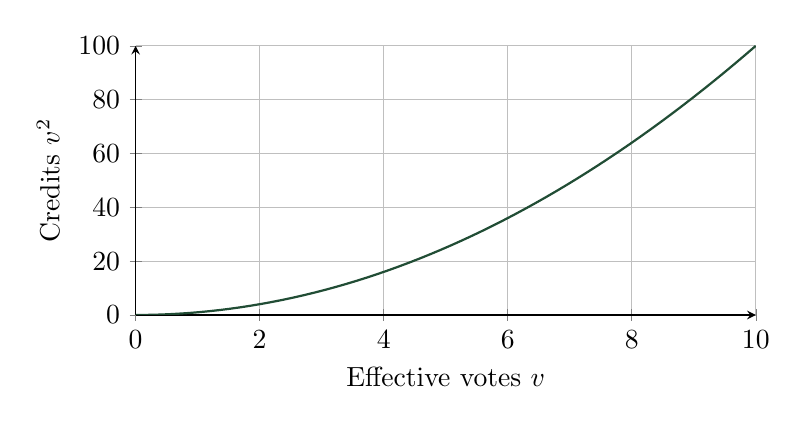
\begin{tikzpicture}
\begin{axis}[width=.78\linewidth,height=5cm,xmin=0,xmax=10,ymin=0,ymax=100,
 xlabel={Effective votes $v$},ylabel={Credits $v^2$},axis lines=left,grid=major]
\addplot[VotingGreen,thick,domain=0:10,samples=60]{x^2};
\end{axis}
\end{tikzpicture}
\end{center}

\section{What the mechanism does and does not establish}
Quadratic voting is studied as a mechanism under assumptions about preferences, payments, and strategic behavior.\cite{quadratic} This implementation is a local nonnegative credit-allocation counter with a top-$k$ selection rule. It does not implement cash transfers, signed opposition votes, rebates, or an equilibrium solver.

A small optimization problem clarifies one intuition. Suppose, as a separate continuous approximation, that a voter wants to maximize the linear influence objective $\sum_c u_c v_c$ under $\sum_c v_c^2\leq B$, with $u_c\geq0$. The Lagrangian is
\[
\mathcal L(v,\lambda)=\sum_cu_cv_c-\lambda\left(\sum_cv_c^2-B\right).
\]
For positive $u_c$, the first-order condition gives $v_c=u_c/(2\lambda)$. Enforcing the budget yields
\[
v_c=\frac{\sqrt B\,u_c}{\sqrt{\sum_du_d^2}},\qquad
x_c=v_c^2=\frac{B\,u_c^2}{\sum_du_d^2}.
\]
Effective votes are proportional to $u_c$ in this surrogate problem; \emph{credits spent are proportional to squared} $u_c$. That calculation is not a proof of truthful reporting for this package's discrete top-$k$ election. The probability of changing an outcome, other voters' behavior, and how preferences enter the payoff have all been left out.

\section{A three-person credit panel}
Use a new unit-weight panel to isolate the effect of concentration. The first person spends everything on Library. The other two distribute points between Shelters and Trees. We select two projects.
\begin{lstlisting}[style=votingrun]
voting voter add credit_1 "Concentrated credit voter"
voting voter add credit_2 "Distributed credit voter 1"
voting voter add credit_3 "Distributed credit voter 2"
voting election add credits "Two priorities from credits" --ballot-type allocated --seats 2 --budget 100
voting election add-option credits library
voting election add-option credits shelters
voting election add-option credits trees
voting election open credits
voting ballot allocate credits credit_1 library=100
voting ballot allocate credits credit_2 shelters=64 trees=36
voting ballot allocate credits credit_3 shelters=49 trees=51
voting count compare credits
\end{lstlisting}
\generated{credit-totals}
Cumulative totals favor Shelters and Library. Quadratic totals favor Shelters and Trees. In particular, Library gets $\sqrt{100}=10$ effective votes; Shelters gets $\sqrt{64}+\sqrt{49}=15$; Trees gets $\sqrt{36}+\sqrt{51}\approx13.141$. There is no raw-total tie behind this difference.
\generated{credit-methods}
The two outcomes answer different aggregation questions. The quadratic result values support distributed across two people more highly than the raw sum does here. It does not establish that Trees yields more money-valued social benefit than Library.

\section{Method of Equal Shares}
Equal shares uses allocations as cardinal utilities $u_i(c)$ for deciding how to pay for unit-cost candidates. A separate virtual budget gives each voter a share of the available $k$ units. With unit weights, that initial share is $b_i=k/n$. In the implemented weighted extension it is
\[
b_i=\frac{k w_i}{W}.
\]
For each remaining candidate $c$, seek the smallest price per utility $\rho_c$ such that
\[
\sum_i\min\{b_i,\rho_c u_i(c)\}=1.
\]
Only positive-utility supporters can pay. If their remaining budgets sum to less than one, $c$ is unaffordable. Among affordable candidates, elect the one with smallest $\rho_c$ and charge each supporter
\[
p_i(c)=\min\{b_i,\rho_c u_i(c)\},\qquad
b_i\leftarrow b_i-p_i(c).
\]
Then repeat for another seat. The cardinal construction and its generalizations are discussed by Peters, Pierczy\'nski, and Skowron.\cite{equalshares}

\subsection{Finding the price}
For a fixed $c$, sort supporters by their cap thresholds $b_i/u_i(c)$. Before anyone is capped, the candidate price would be $1/\sum_i u_i(c)$. If that price would overcharge a supporter's remaining budget, cap that supporter, subtract its full budget from the outstanding cost, and solve again using the uncapped utility sum:
\[
\rho_c=\frac{1-\text{already capped budget}}{\text{uncapped utility sum}}.
\]
The sorted scan identifies the first feasible price. This avoids testing an arbitrary grid of possible prices. The package uses a small numerical tolerance when checking affordability and equal prices.

In the three-person panel, each person starts with $2/3$. Library's only supporter cannot alone afford its unit cost. Shelters and Trees initially have two supporters and are affordable. Shelters is cheaper per utility and is selected. The remaining virtual budget cannot fund another candidate from its positive-utility supporters. The package then fills the remaining seat by raw utility totals, which selects Library.

\subsection{Completion and weights are substantive choices}
When no candidate is affordable before all seats are filled, this package completes the committee using the largest remaining raw point totals. Such rounds have \code{completion: utilitarian}; the result also lists \code{completed_seats}. Report that distinction instead of attributing every selected member to the affordability stage.

The virtual candidate cost is always one. This is not a solver for a collection of projects with heterogeneous dollar costs. Also, in the weighted implementation, $w_i$ changes the initial virtual budget, while the price equation uses $u_i(c)$ without an additional weight multiplier. A weighted agent is therefore not automatically equivalent to several identical unit-weight agents in equal shares. The examples in this chapter use explicit unit weights to avoid conflating those interpretations.

\section{A cohesive minority and three seats}
For a second committee question, add Garden as a fifth town proposal. Four unit-weight panelists support Library, Shelters, and Trees; two support Playground and Garden. Each has 100 credits. The example is designed so the minority's raw support is divided between two options.
\begin{lstlisting}[style=votingrun]
voting option add garden "Garden" --type proposal
voting voter add panel_1 "Committee panelist 1"
voting voter add panel_2 "Committee panelist 2"
voting voter add panel_3 "Committee panelist 3"
voting voter add panel_4 "Committee panelist 4"
voting voter add panel_5 "Committee panelist 5"
voting voter add panel_6 "Committee panelist 6"
voting election add representation "Three representative priorities" --ballot-type allocated --seats 3 --budget 100
voting election add-option representation library
voting election add-option representation shelters
voting election add-option representation trees
voting election add-option representation playground
voting election add-option representation garden
voting election open representation
voting ballot allocate representation panel_1 library=34 shelters=33 trees=33
voting ballot allocate representation panel_2 library=34 shelters=33 trees=33
voting ballot allocate representation panel_3 library=34 shelters=33 trees=33
voting ballot allocate representation panel_4 library=34 shelters=33 trees=33
voting ballot allocate representation panel_5 playground=50 garden=50
voting ballot allocate representation panel_6 playground=50 garden=50
voting count compare representation
\end{lstlisting}
\generated{representation-methods}
The cumulative totals for the majority's three options are 136, 132, and 132, exceeding each minority option's 100. That selects three majority-supported projects. In equal shares each panelist starts with $3/6=1/2$ of virtual budget. The two minority panelists can together fund one project; their budget cannot be spent on projects for which they report zero utility.
\generated{mes-rounds}
This example demonstrates a representation mechanism. It is not a general theorem that every possible cardinal profile, weighted extension, or completion policy satisfies every proportionality axiom. Distinguish the observed example, the exact implemented rule, and the assumptions of any theorem being cited.

\section{Exercises}
\begin{enumerate}
\item Show that changing a voter's budget from 100 to 400 multiplies its quadratic support by two if it preserves all spending proportions.
\item In the three-person panel, compute the initial equal-shares price for Shelters. What remains of the two supporters' budgets after funding it?
\item Why can an equal-shares candidate with the highest raw utility total be initially unaffordable?
\item Replace both minority ballots by a single row of weight two in a fresh copy. Compare its payment equation with two separate rows. Explain why a budget share and a utility multiplicity are different operations.
\end{enumerate}

\chapter{Collect, validate, revise, and explain}
\label{chap:practice}
\section{Make the instrument match the question}
Before collecting real preferences, specify the decision, eligible options, eligible voters, ballot type, seats, tie convention, and meaning of missing answers. For allocated ballots, specify the credit budget. For grades, specify labels from worst to best. For limited voting, set the approval limit before collection.

Configuration is inspectable and editable through the CLI:
\begin{lstlisting}
voting election show credits
voting election configure credits --budget 100 --seats 2
voting election configure limited --approval-limit 2
voting election configure grades --grade reject --grade poor --grade fair --grade good --grade excellent
\end{lstlisting}
Changing a constraint after collection can make earlier ballots invalid. Revalidate and explain which ballots the new rule excludes. Do not treat a count made under a changed scale as the same measurement instrument.

\section{Importing existing responses}
For a JSON import, the outer object can identify the election and ballot type, and each row supplies a voter ID and the answer field corresponding to that type:
\begin{lstlisting}[language={}]
{
  "election_id": "credits",
  "ballot_type": "allocated",
  "rows": [
    {"voter_id": "credit_1",
     "answer": {"allocations": {"library": 70, "trees": 30}}}
  ]
}
\end{lstlisting}
Save a file like this as \code{responses.json}, then use:
\begin{lstlisting}
voting ballot import --election credits --from responses.json
voting ballot validate credits
\end{lstlisting}
The JSON importer supports all six ballot types. The answer keys are \code{choice}, \code{ranking}, \code{approved}, \code{scores}, \code{grades}, and \code{allocations}. Numeric values must be JSON numbers. An explicit \code{"approved": []} records an approval abstention; a missing approval answer is not silently converted into one.

Imports report invalid rows under \code{skipped_detail}. A rejected row does not replace the voter's previous valid ballot. Unknown voters can be recorded with a warning but cannot count until registered; \code{--register-voters} registers valid unknown respondents at weight one. Inspect who was added instead of assuming an imported respondent identifier is an eligibility decision.

\section{Errors as executable examples}
These four orange listings intentionally fail. The builder checks that each returns an error envelope and records that failure in the command transcript.
\begin{lstlisting}[style=votingerror]
voting ballot allocate credits credit_1 library=101
voting ballot allocate credits credit_1 library=100 trees=-1
voting ballot grade grades readers library=A
voting count run ranked --method score
\end{lstlisting}
\generated{validation}
The first violates the 100-credit budget. The second uses a negative allocation. The third uses a grade outside the stored scale. The fourth asks a score counter to analyze ranked ballots, which contain no scores.

The first person's existing credit ballot still spends 100 on Library. A command's failure is not permission to mutate a different record or guess what the voter intended.
\begin{lstlisting}[style=votingrun]
voting ballot validate credits
voting ballot list --election credits --latest
\end{lstlisting}
When counting previously stored data, invalid ballots are excluded with warnings. With no valid ballots the package declares no winner. A successfully executed count can still contain data-quality warnings; success means the command completed.

\section{Ballot revisions and stale results}
Create a small separate ranked election using the three credit panelists. This exercise changes one person's answer rather than changing an entire weighted group.
\begin{lstlisting}[style=votingrun]
voting election add revision "A preference changes" --ballot-type ranked
voting election add-option revision library
voting election add-option revision shelters
voting election add-option revision trees
voting election open revision
voting ballot rank revision credit_1 library shelters trees
voting ballot rank revision credit_2 library shelters trees
voting ballot rank revision credit_3 shelters trees library
voting count run revision --method irv
voting status
voting ballot rank revision credit_2 shelters trees library
voting status
voting count run revision --method irv
voting election close revision
voting status
\end{lstlisting}
Initially Library has two of three first preferences. After the second person's revision, Shelters has two. The second ballot supersedes the older ballot for that voter only in \code{revision}; their allocated ballot in \code{credits} is unaffected.
\generated{revision-history}
The first saved count remains on disk. After the recast it is stale, because its input fingerprint no longer matches the current ballot set. Recounting creates a current result. Closing the election does not erase the count or send the project back to setup.

\code{status} reports each election independently. \code{next} prioritizes unfinished work and names the appropriate ballot command. Results from an unrelated election do not complete a new one. Results from older package versions without an input fingerprint should be recounted rather than presumed current.

\section{Reading plots responsibly}
The package can export SVG figures:
\begin{lstlisting}
voting plot ranks ranked
voting plot methods --election ranked
voting plot scores <borda_result_id>
voting plot pairwise <schulze_result_id>
\end{lstlisting}
Replace angle-bracket placeholders with actual saved result IDs. A ranks plot summarizes validated latest ballots. A pairwise plot shows row-over-column margins. A score plot needs a method exposing numeric totals; it is not the same display as an ordinal grade median.

Always restrict a method comparison to a clearly identified election. Saved counts can reflect different collection dates, seat overrides, or eligibility settings. A color grid alone cannot establish that the input snapshots match. For multi-seat counts, a finishing position of two may still be elected; read the winner sets, not just the darkest cell.

\section{Optional human and AI fielding}
The base package's local examples need no EDSL installation. To construct synthetic or hosted surveys, install the documented \code{humanize} extra. Those integrations support ranked, single-choice, approval, and score ballots. Grade and allocated exercises in this edition use direct entry or JSON import.

Synthetic fielding builds a Jobs package with the survey, eligible voter agents, and a model. The voting package does not execute the model:
\begin{lstlisting}
voting survey generate ranked --model gpt-5.5 --service openai
voting --human survey show ranked
ep run --jobs .voting/output/survey_ranked.jobs.ep --output .voting/output/survey_ranked.results.ep
voting ballot import --election ranked --from-results .voting/output/survey_ranked.results.ep
\end{lstlisting}
Inspect the questions, personas, model, and expected call count before external execution. Model-generated preferences are a distinct data source from human responses. Do not describe synthetic agents as a sample of residents, or take agreement between several models as measured public opinion.

For a hosted human survey:
\begin{lstlisting}
voting survey humanize ranked
voting survey publish ranked
voting survey responses ranked
voting ballot import --election ranked --from-results .voting/output/humanize_responses_ranked.ep --register-voters
\end{lstlisting}
Publishing creates a hosted survey. Without email delivery, share its respondent URL. With registered eligible voters and an email trait, the package can prepare and send unique invitation links:
\begin{lstlisting}
voting survey humanize ranked --email-trait email
voting survey publish ranked
voting survey email ranked --name "Neighborhood priorities"
\end{lstlisting}
These are alternative fielding instructions, not steps executed by the manual. They require appropriate voter information and service authentication. Survey generation excludes ineligible options, reference entries, and ineligible voters; publishing a previously generated job does not retroactively rebuild it when eligibility changes.

\clearpage
\section{A report that makes the decision understandable}
Report the question and who answered it, then the instrument and how invalid or missing responses were treated. Name the counting rule, seats, quota or score convention, and tie handling. Present the winner alongside enough diagnostics to explain it: an elimination path, pairwise matrix, score/runoff decomposition, or payment rounds.

Compare methods on the same instrument when possible, and state explicitly when a comparison uses newly elicited scores or approvals. Describe the extent of disagreement without counting method names as independent evidence. Aliases, such as \code{qv} and \code{quadratic}, are the same algorithm.

\section{Exercises}
\begin{enumerate}
\item Inspect the before-and-after revision count records. Which ballot IDs differ?
\item Why is a zero-approval ballot different from a missing response, even if neither adds approval points?
\item Draft a four-sentence report of the town's ranked election. Include plurality, IRV, the Condorcet winner, and one limitation of the fictional data.
\end{enumerate}

\chapter{A working reference and a research agenda}
\label{chap:reference}
\section{Match methods to available information}
\begin{longtable}{p{.19\linewidth}p{.40\linewidth}p{.30\linewidth}}
\toprule Ballot & Core compatible methods & What cannot be recovered\\\midrule\endhead
Single choice & FPTP, simple majority, SNTV, runoff, approval & Lower preferences for an eliminated choice\\
Ranked & FPTP, simple majority, Borda, IRV, STV, Bucklin, runoff, Copeland, minimax, ranked pairs, Schulze, Kemeny--Young & Cardinal distances or an approval threshold\\
Approval & Approval, block, limited & Ordering or intensity among approved options\\
Score & Score, STAR & A unique categorical grade scale or credit budget\\
Grade & Majority judgment & Cardinal distances between labels\\
Allocated & Cumulative, quadratic, equal shares & Actual project costs or a model of strategic behavior\\
\bottomrule
\end{longtable}
Compatibility is necessary but not sufficient. A method can also reject a seat count or approval limit. Default \code{count compare} reports methods it skips; an explicit incompatible method list fails before saving any comparison results. Read the reason instead of silently changing the instrument until every name runs.

\section{Aliases do not add independent evidence}
The following table is generated from the package's registry. It groups accepted names by the same underlying algorithm function. There are \MethodNameCount{} registered names in this edition, covering \AlgorithmCount{} functions.
\generated{aliases}
STV with one seat delegates to IRV, and approval-family methods share a tally while imposing different legal ballot limits. Even distinct function names need not produce independent answers. A claim that ten methods agree should identify which rules were actually compared.

\section{Computational scale}
Let $n$ be the number of countable ballot rows and $m$ the number of eligible options. These bounds describe the current direct implementations, not the best possible algorithm for every rule:
\begin{longtable}{p{.28\linewidth}p{.24\linewidth}p{.38\linewidth}}
\toprule Calculation & Typical upper-bound work & Main source of cost\\\midrule\endhead
Plurality & $O(n+m\log m)$ & Scan choices and sort totals\\
Approval, score, Borda & $O(nm+m\log m)$ & Read supplied option values\\
Pairwise matrix & $O(nm^2)$ & Compare every ordered pair on each ballot\\
IRV & $O(nm^2)$ & Repeated active-choice scans\\
STV & $O(nm^2)$ plus sorting & Transfers and eliminations across rounds\\
Bucklin & $O(nm^2)$ & Recount prefixes at increasing depth\\
Ranked pairs & Up to $O(m^4)$ after pairwise counts & Graph search for each candidate edge\\
Schulze & $O(nm^2+m^3)$ & Pairwise counts and max--min closure\\
Kemeny--Young & $O(nm^2+m!m^2)$ & Enumerate and score permutations\\
Equal shares & About $O(kmn\log n)$ & Sort supporters for candidate prices each round\\
\bottomrule
\end{longtable}
For most small teaching elections, reading project files and starting CLI processes dominate. For Kemeny, the factorial quickly dominates everything else. Weighted rows can reduce file counts, but the interpretation of grouping must still be appropriate to the method.

Majority judgment uses weighted grade histograms and skips blocks of repeated median removal. Its work depends on grade transitions and integer arithmetic, rather than allocating one list element per unit of voting weight.

\section{Questions to ask of an algorithm}
\emph{Majority consistency.} Does an option ranked first by a strict majority necessarily win? Work through the package's rule rather than transferring the property from a similar name.

\emph{Condorcet consistency.} Does the rule choose a candidate that beats every other candidate when one exists? The main example makes clear that IRV and the pairwise methods answer differently even with complete ballots.

\emph{Monotonicity.} Could raising an option on a ballot make its outcome worse? An elimination path can change discontinuously. A fixed profile illustrates an outcome; proving a property requires considering all permitted profiles.

\emph{Representation.} Does the committee give substantial groups a voice, or does it concentrate on the largest aggregate totals? Specify the axiom and the ballot domain before treating either as mathematically equivalent to fairness.

\emph{Neutrality and ties.} Does renaming an option change the outcome? Lexicographic resolution deliberately uses IDs in tied situations. Save and disclose the tie convention.

\emph{Strategy.} What can a participant gain by changing their message? A direct count is not a behavioral or equilibrium model. Strategic simulations need a specified information structure, utility function, and feasible deviations.

\section{Selected answers and calculations}
\textbf{Chapter 1.} Library leads first choices, but 42 is below the majority threshold of 50. Trees beats Shelters by $42+17=59$ to $26+15=41$, and beats Library by $26+17+15=58$ to 42.

\textbf{Chapter 3.} Borda totals are Library 126, Shelters 184, Trees 176, and Playground 114, summing to 600. If Families list only Playground, its elimination exhausts 15 and leaves 85 continuing weight. Trees is then eliminated, transferring 17 to Shelters. Shelters has 43 against Library's 42 and wins with a majority of 85, while having less than half the original 100.

\textbf{Chapter 4.} Trees has Copeland score 3 and minimax score 0. In the symmetric cycle, the package considers Library over Shelters before Shelters over Trees, then skips Trees over Library because it would close the cycle. The strongest path in each direction between Library and Trees has strength 2.

\textbf{Chapter 5.} Library's residual transfer is $42(8/42)=8$, retaining 34. In a two-seat result, the runner-up is the first candidate outside the two-person winner set.

\textbf{Chapter 6.} If only one person scores Library 10 while two score Shelters 6, Library has the greater reported average but Shelters the greater sum. The fractional-weight grade example elects Trees; both grades retain positive weight.

\textbf{Chapter 7.} Shelters' initial equal-shares price in the three-person credit panel is $1/113$. The two payments are $64/113$ and $49/113$, both below $2/3$. The supporters retain $2/3-64/113$ and $2/3-49/113$, whose sum is $1/3$. That cannot fund another unit-cost candidate by itself.

\textbf{Chapter 8.} A valid empty approval ballot is a submitted abstention and supersedes an earlier ballot. A missing response should not erase a prior recorded answer merely because a field was absent.

\section{Extend the example}
Start a fresh manual build before changing a profile. Useful follow-ups include perturbing one unit-weight ballot, truncating rankings systematically, changing an approval limit, scaling all score responses together, changing only one person's score scale, and comparing representative committees under different cardinal utility assumptions.

For each experiment, write the hypothesis first, preserve the baseline, and report the change in both inputs and outputs. If studying uncertainty, introduce an explicit sampling or behavioral model. Recounting a fixed ballot file with several deterministic rules is a sensitivity analysis over rules, not a confidence interval for public support.

\appendix
\chapter{Results from this build}
Each row is a saved count from the executed listings. Repeated counts of the same election, method, and seat count are represented by their latest result here; the complete history remains in \code{results.json}. Results from different elections can answer different questions and must not be mistaken for alternative counts of an unchanged instrument.
\generated{all-results}
\chapter{Executed command transcript}
Start in a fresh exported manual directory. The transcript initializes \code{study} and enters it once. Commands marked as expected errors demonstrate validation and intentionally exit nonzero. Executing this over an existing project will encounter duplicate IDs; rebuild into a fresh directory instead.
\IfFileExists{generated/commands.txt}{\lstinputlisting{generated/commands.txt}}{No commands were executed for this sources-only edition.}
\begin{thebibliography}{9}
\bibitem{handbook}
Felix Brandt, Vincent Conitzer, Ulle Endriss, J\'er\^ome Lang, and Ariel D. Procaccia, editors.
\emph{Handbook of Computational Social Choice}. Cambridge University Press, 2016.
\url{https://procaccia.info/wp-content/uploads/2020/03/comsoc.pdf}.

\bibitem{rankedpairs}
Cynthia Maushagen, David Niclaus, Paul N\"usken, J\"org Rothe, and Tessa Seeger.
\emph{Toward Completing the Picture of Control in Schulze and Ranked Pairs Elections}.
Proceedings of IJCAI, 2024. See the definitions of ranked pairs and its locked graph.
\url{https://www.ijcai.org/proceedings/2024/0326.pdf}.

\bibitem{schulze}
Markus Schulze. \emph{The Schulze Method of Voting}, 2018.
\url{https://arxiv.org/abs/1804.02973}.

\bibitem{star}
STAR Voting. \emph{STAR Voting Technical Specifications}, version 1.3.
\url{https://assets.nationbuilder.com/unifiedprimary/pages/501/attachments/original/1734730674/STAR_Voting_Technical_Specifications_V1.3.pdf}.

\bibitem{majorityjudgment}
Michel Balinski and Rida Laraki. A theory of measuring, electing, and ranking.
\emph{Proceedings of the National Academy of Sciences}, 104(21):8720--8725, 2007.
\url{https://doi.org/10.1073/pnas.0702634104}.

\bibitem{quadratic}
Steven P. Lalley and E. Glen Weyl. Quadratic Voting: How Mechanism Design Can Radicalize Democracy.
\emph{AEA Papers and Proceedings}, 108:33--37, 2018.
\url{https://doi.org/10.1257/pandp.20181002}.

\bibitem{equalshares}
Dominik Peters, Grzegorz Pierczy\'nski, and Piotr Skowron.
\emph{Proportional Participatory Budgeting with Additive Utilities}, version 2, October 2022.
See Section 3 for the Method of Equal Shares.
\url{https://dominik-peters.de/publications/equal-shares.pdf}.
\end{thebibliography}

\end{document}
